\section{Generating referring expressions} \label{sec:gre}

Now we apply description logic to GRE.  The core claim of this paper
is that the GRE problem can be viewed as the problem of computing a
formula of description logic whose extension is exactly a given set of
individuals.

\medskip
\noindent
{\small
\begin{center}
\begin{tabular}{ll} \hline
\multicolumn{2}{l}{
\textsc{$\gL$-GRE Problem}}\\ \hline
\ \ Input: & A model $\gM$ and a set $A \subseteq \Delta^\gM$.\\
\ \ Output: & A formula $\varphi \in \gL$ such that $|\varphi|^\gM = A$\\
& \hspace*{0.5cm} (if such a formula exists).\\ \hline
\end{tabular}
\end{center}}
\medskip

In the examples above, it is because $\mathsf{flower} \sqcap \exists
\mathsf{in}. \mathsf{hat}$ denotes exactly $\{f_2\}$ that we can say
``the flower in the hat'' to refer to $f_2$.  This generalizes the
common view of GRE as attribute selection \cite{Dale1995}: From our
perspective, a bag of attributes is simply a conjunction of atoms.
However, more expressive approaches to GRE fit into our framework as
well; for example, relational expressions as in
\newcite{dale91:_gener_refer_expres_invol_relat} are formulas of \el.
Different approaches will deliver different REs, and indeed will be
able to build REs at all in different circumstances; this reflects the
differences between the DL languages they use to represent their REs
in.  This idea provides a unified perspective for comparing different
GRE approaches, and we will discuss how to see several further
approaches in Section~\ref{sec:related}.

For the rest of this paper, we assume that we are generating a
singular RE, i.e.\ $A$ will generally be a singleton set.  In this
case, we will only be able to generate a formula that denotes exactly
$A = \{a\}$ (i.e., a RE that uniquely refers to $a$) iff there is no
other individual $b$ that is bisimilar to $a$; otherwise, any formula
that is satisfied by $a$ is also satisfied by $b$.  This is why there
is no RE that uniquely refers to $t_2$ in Fig.~\ref{fig:dale-haddock}a
and only uses the relations ``on'' and ``in'' (and not their
inverses).  In other words, $A$ must be a bisimulation class.
Conversely, if we know that $a$ is alone in its bisimulation class, we
know that there is a concept that describes only $a$ and nothing
else.  This means that we can recast the problem of generating
referring expressions as the problem of computing the bisimulation
classes of a model.

In the rest of this section, we will present algorithms that compute
the bisimulation classes of a given model for \alc\ and \el, along
with a characteristic formula for each class.  These algorithms
efficiently compute \emph{all} bisimulation classes of a model, and
not just the one for some target referent.  In effect, they compute
REs for all individuals in some model at the same time.  The REs
generated by the \el\ algorithm correspond to the relational REs
generated e.g.\ by \newcite{dale91:_gener_refer_expres_invol_relat}
(but without any danger of infinite regress), whereas the REs
generated by the \alc\ algorithm can freely use negation as well.



\subsection{Bisimulation classes for \alc and \el}

There is substantial literature on the topic of computing the
\alc-bisimulation classes of a given model efficiently
\cite{hopc:algo71,paig:thre87,dovier04:_effic_algor_for_comput_bisim_equiv}.
However, these algorithms will only compute the bisimulation classes
themselves. We extend the \newcite{hopc:algo71} algorithm in such a
way that it computes, for each bisimulation class, also a formula that
denotes exactly this class.  We can then use these formulas as
representations of the REs.

The pseudocode for our \alc\ algorithm is shown as
Algorithm~\ref{algo:bisim-l} and Algorithm~\ref{algo:bisim-add-alc}.
Given a model $\gM=(\Delta^\gM, |\cdot|^\gM)$, the algorithm computes
a set $\RE$ of $\alc$ formulas such that the set $\{|\varphi|^\gM \mid
\varphi \in \RE\}$ is the set of \alc-bisimulation classes of $\gM$.
The algorithm starts with $\RE = \{\top\}$ (where $\interp{\top} =
\Delta^\gM$), and successively refines $\RE$ by making its elements
denote smaller and smaller sets.  It maintains the invariant that at
the start and end of every iteration, $\{|\varphi|^\gM \mid \varphi
\in \RE\}$ is always a partition of $\Delta^\gM$.  The algorithm
iterates over all propositional and relational symbols of the
signature to construct new formulas until either all formulas in $\RE$
denote singletons (i.e., there is only one individual that satisfies
them), or no progress has been made in the previous iteration.  In
each iteration, it calls the procedure add$_\alc$($\varphi$, $\RE$),
which intersects $\varphi$ with any formula $\psi \in \RE$ which does
not denote a singleton and which is not equivalent to $\varphi$ and to
$\neg \varphi$. In this case, it replaces $\psi$ in $\RE$ by $\psi
\sqcap \varphi$ and $\psi \sqcap \neg \varphi$.


\begin{algorithm}[t]
\dontprintsemicolon
\caption{Compute $\mathcal{L}$-bisimulation classes}
\label{algo:bisim-l}
\KwIn{A model $\gM = (\Delta^\gM, |\cdot|^\gM)$}
\KwOut{A set \RE of formulas  such that
$\{|\varphi|^\gM \in \RE\}$ is the set of $\mathcal{L}$-bisimulation
classes of $\gM$.}

$\RE \leftarrow \{\top\}$

\For{$p \in \prop$}{
      add$_\mathcal{L}(p,\RE)$
   }

\While{for some $\varphi \in \RE, |\varphi|^\gM>1$}{
   \For{$\varphi \in \RE, R \in \rel$}{
         add$_\mathcal{L}(\exists R.\varphi,\RE)$
   }
   \If{made no changes to \RE}{
      exit
      }
}
\end{algorithm}

The \alc\ algorithm is capable of computing the \alc-bisimulation
class of the model very efficiently, in time $O(nm)$ where $n$ is the
number of individuals in the domain, and $m$ is the number of pairs of
individuals that are related by some relation.  However, it will
freely introduce negations in the case distinctions, which can make
the resulting formula hard to realize (see also
Section~\ref{sec:discussion-realization}).  This is why we also
present an algorithm for the \el-bisimulation classes; \el\
corresponds to positive relational REs, which are generally easy to
realize.

We obtain the \el\ algorithm by replacing the call to add$_{\alc}$ in
Algorithm~\ref{algo:bisim-l} by a call to add$_{\el}$, which is defined
in Algorithm~\ref{algo:bisim-add-el}.  As before, the algorithm
maintains a set $\RE = \{\varphi_1,\ldots,\varphi_n\}$ of formulas
(this time of \el) such that $\interp{\varphi_1}^\gM \cup \ldots \cup
\interp{\varphi_n}^\gM = \Delta^\gM$, and which it refines
iteratively.  However, where the \alc\ algorithm maintains the
invariant that $\interp{\varphi_1},\ldots,\interp{\varphi_n}$ is a
partition of $\Delta$, we weaken this invariant to the requirement
that there are no $m \geq 2$ pairwise different indices $1 \leq
i_1,\ldots,i_m \leq n$ such that $\interp{\varphi_{i_1}} =
\interp{\varphi_{i_2}} \cup \ldots \cup \interp{\varphi_{i_m}}$.  We
call the formula $\varphi_{i_1}$ \emph{subsumed} if such a
decomposition exists.


Because the \el\ algorithm maintains a weaker invariant for the
classes, it may consider more of these classes simultaneously.  Prima
facie, this means that it has worst-case exponential runtime, given
that the whole domain has an exponential number of subsets.  However,
it is possible that a more careful analysis of the combinatorics of
the considered subsets will reveal that the algorithm is actually
polynomial.


% \begin{figure}
%   \centering
%   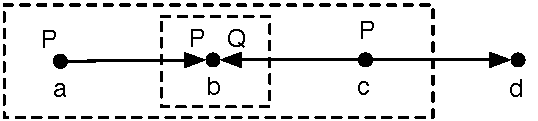
\includegraphics[width=\columnwidth]{pic-el-vs-alc}
%   \caption{Illustrating the difference between \el\ and \alc.}
%   \label{fig:el-vs-alc}
% \end{figure}

\subsection{Some Examples}\label{sec:examples}

We will now see what our algorithms do in some interesting
examples. Consider the model shown in
Fig.~\ref{fig:dale-haddock}a, which is taken from
\newcite{dale91:_gener_refer_expres_invol_relat}, and
let's run the $\el$ algorithm.


\begin{algorithm}[t]
\caption{add$_\alc(\varphi,\RE)$}
\label{algo:bisim-add-alc}
\For{$\psi \in \RE$ with $|\psi|^\gM > 1$}{
   \If{$|\psi \sqcap \varphi|^\gM \not = \emptyset$ and
       $|\psi \sqcap \neg \varphi|^\gM \not = \emptyset$}{
         add $\psi \sqcap \varphi$ and
               $\psi \sqcap \neg \varphi$ to \RE \;
         remove $\psi$ from \RE \;
      }
   }
\end{algorithm}
%
\begin{algorithm}[t]
\dontprintsemicolon
\caption{add$_\el$($\varphi$, $\RE$)}
\label{algo:bisim-add-el}
\For{$\psi \in \RE$ with $|\psi|^\gM > 1$}{
  \If{$\psi \sqcap \varphi$ is not subsumed in $\RE$ {\bf and}
    $|\psi \sqcap \varphi|^\gM \neq \emptyset$ {\bf and}
    $|\psi \sqcap \varphi|^\gM \neq |\psi|^\gM$}{
    add $\psi \sqcap \varphi$ to $\RE$ \;
    remove subsumed concepts from $\RE$\;
  }
}
\end{algorithm}

The algorithm starts with $\RE = \{\top\}$.  In the first loop, it
adds the formulas $\mathsf{floor}$, $\mathsf{bowl}$, $\mathsf{cup}$,
and $\mathsf{table}$, and then removes $\top$ because it is now
subsumed.  Not all of these formulas denote singletons; for instance,
$|\mathsf{cup}|^\gM$ contains two individuals.  So we iterate over the
relations to refine our formulas.  After the first iteration over the
relations, we have $\RE = \{ \mathsf{floor}, \mathsf{bowl} \sqcap
\exists \mathsf{on}.\mathsf{floor}, \mathsf{bowl} \sqcap \exists
\mathsf{on}.\mathsf{table}, \mathsf{cup}, \mathsf{table} \}$. Notice
that $\mathsf{bowl}$ has become subsumed, but we haven't distinguished
the cups and tables further.

Now we can use the distinction between the bowls to distinguish the
cups in the second iteration.  The result of this is $\RE = \{
\mathsf{floor}, \mathsf{bowl} \sqcap \exists
\mathsf{on}.\mathsf{floor}, \mathsf{bowl} \sqcap \exists
\mathsf{on}.\mathsf{table}, \mathsf{cup} \sqcap \exists
\mathsf{in}. (\mathsf{bowl} \sqcap \exists
\mathsf{on}.\mathsf{floor}), \mathsf{cup} \sqcap \exists
\mathsf{in}. (\mathsf{bowl} \sqcap \exists
\mathsf{on}.\mathsf{table}), \mathsf{table} \}$.

At this point, all formulas except $\mathsf{table}$ denote singletons,
and further iterations don't allow us to refine $\mathsf{table}$; so
the algorithm terminates.  Each of the singleton bisimulation classes
is represented by a characteristic formula; for instance, $\RE$ tells
us that $\mathsf{cup} \sqcap \exists \mathsf{in}. (\mathsf{bowl}
\sqcap \exists \mathsf{on}.\mathsf{table})$ is only satisfied by
$c_2$, so we may refer to $c_2$ as ``the cup in the bowl on the
table''.  Notice that the algorithm didn't focus on any particular
individual; it simultaneously generated REs for all individuals except
for the two tables.


\begin{figure}[t]
  \centering
  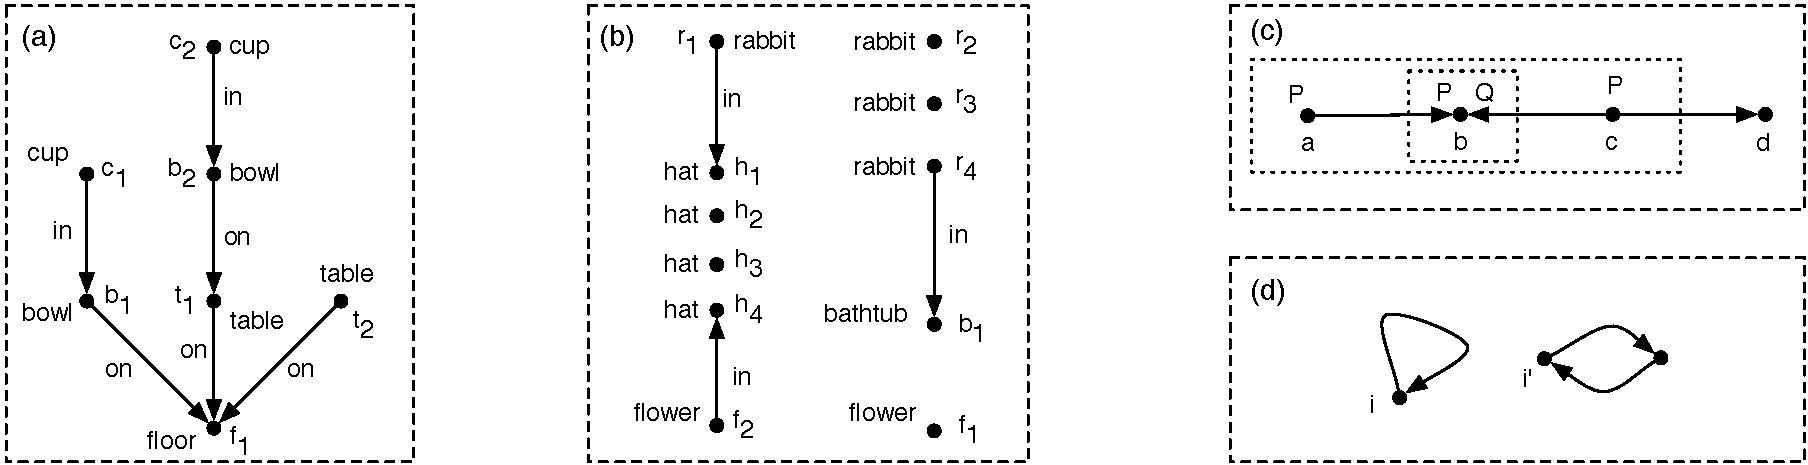
\includegraphics[width=\columnwidth]{pic-dale-haddock}
  \caption{(a) The \newcite{dale91:_gener_refer_expres_invol_relat}
    scenario; (b) the \newcite{Stone1998a} scenario.}
  \label{fig:dale-haddock}
\end{figure}

The \el\ algorithm has a harder time with the example in
Fig.~\ref{fig:dale-haddock}b \cite{Stone1998a}.  While it will
correctly identify $r_1$ as ``the rabbit in the hat'' and $f_2$ as
``the flower in the bathtub'', it will not be able to compute a
RE for $f_1$; indeed, the algorithm terminates with $\RE$ containing
both $\mathsf{flower}$ and $\mathsf{flower} \sqcap \exists
\mathsf{in}.\mathsf{hat}$.  By contrast, the \alc\ algorithm will
split $\mathsf{flower}$ into the two new formulas $\mathsf{flower}
\sqcap \exists \mathsf{in}.\mathsf{hat}$ and $\mathsf{flower} \sqcap
\neg \exists \mathsf{in}.\mathsf{hat}$, generating a unique RE for
$f_1$ as well.



%%% Local Variables: 
%%% mode: latex
%%% TeX-master: "dl-gre-08"
%%% End: 

% \begin{algorithm}[t]
% \dontprintsemicolon
% \caption{\el\ bisimulation classes}
% \label{algo:bisim-el}
% \KwIn{A model $\gM = (\Delta^\gM, |\cdot|^\gM)$}
% \KwOut{A set \RE of pairs $(\varphi,|\varphi|^\gM)$ such that
% $\{S \mid (\varphi,S) \in \RE\}$ is the set of $\el$-bisimulation
% classes of $\gM$.}
% \RE $\leftarrow \{(\top,\Delta^\gM)\}$ \;
% \For{$p \in \prop$}{
%   add$_\el$(p, \RE) \;
% }
% \While{for some $(\varphi,S) \in \RE$, $|S| > 1$}{
%   \For{$(\varphi,S) \in$ \RE, $R \in \rel$}{
%     add$_\el$($\exists R.\varphi$, \RE) \;
%   }
%   \If{made no changes to $\RE$}{
%     exit\;
%   }
% }
% \end{algorithm}